\documentclass{book}

\usepackage{amsmath}
\usepackage{amssymb}
\usepackage{amsxtra}
\usepackage{graphicx}
\usepackage{listings}
\usepackage[hidelinks]{hyperref}
\usepackage[T1]{fontenc}

\newcommand{\refchapter}[1]{Chapter~\ref{#1}}
\newcommand{\refsec}[1]{Section~\ref{#1}}
\newcommand{\refeqn}[1]{Equation~(\ref{#1})}
\newcommand{\reffig}[1]{Figure~\ref{#1}}

\title{\bf Software Lab\\ Computational Engineering Science \\
{\large C++ UI design for NAG Optimization Modelling Suite}\\
{\normalsize Group 6: Maksim Feldman, Yifei Huang, Tran Man Khang, Konstantin Korkin, Ziya Valiyev}} 

\author{Uwe Naumann\footnote{Informatik 12: Software and Tools for Computational Engineering, RWTH Aachen University, {\tt info@stce.rwth-aachen.de}}}
\date{
\includegraphics[width=.6\textwidth]{rwth_i12_softw-werkz_en_rgb}}

\begin{document}

\lstloadlanguages{[ISO]C++}
\lstset{basicstyle=\small, numbers=left, numberstyle=\footnotesize,
  stepnumber=1, numbersep=5pt, breaklines=true, escapeinside={/*@}{@*/}}

\pagestyle{headings}

\maketitle

\tableofcontents

\chapter*{Preface}
This report summarizes our work on the topic "C++ UI design for NAG Optimization Modelling Suite", issued by the department of Informatik 12: Software and Tools for Computational Engineering, RWTH Aachen University. Included in the report is a holistic overview about how we developed our C++ interface, from analysis to implementation and testing, as well as a detailed user documentation for guidance on how to use said interface. \\
\newline
Whether it be a structural engineering problem, or perhaps in making financial decision, we often speak of the term \textit{numerical optimization}, i.e. solving a math problem so as to select the most suitable material for constructing a bridge or to gauge the most optimal of money to invest in the right company. Various commercially available programs have been written to this end of mathematically modeling a real life problem and then choosing the best solution. In this project, we were tasked with designing an interface in the C++ programming language for one such program.\\
\newline
As students pursuing a Bachelor in Computational Engineering Science, the topic was appropriate for us, serving as a reinforcement of the prior knowledge we acquired over the course of our study, such as programming in C++, creating UML class diagrams, building system with CMake, and among other skills. At the same time, it offered us an opportunity to expand our horizon in the field of software engineering.\\
\newline
We would like to thank Dr. Johannes Lotz\footnote{\tt \href{mailto:lotz@stce.rwth-aachen.de}{\nolinkurl{lotz@stce.rwth-aachen.de}}} from STCE for his guidance and support throughout the project and Prof. Dr. Uwe Naumann\footnote{\tt \href{mailto:naumann@stce.rwth-aachen.de}{\nolinkurl{naumann@stce.rwth-aachen.de}}} for the overall supervision, without which this could not have come into fruition. 
\chapter{Analysis} \label{ch:analysis}
This chapter goes into the requirements analysis of the project as well as offers brief mathematical knowledge regarding optimization problems.
\section{User Requirements}
Put succinctly, the C++ interface is to be used to define and solve optimization problems.\\
\newline
The user expects the interface to first define an optimization problem based on user-defined objective functions and constraints, then solve said problem without requiring the user to compute the derivatives of the given functions. The interface is to choose the optimal solver based on how the optimization problem is classified.\\
\begin{figure}[!h]
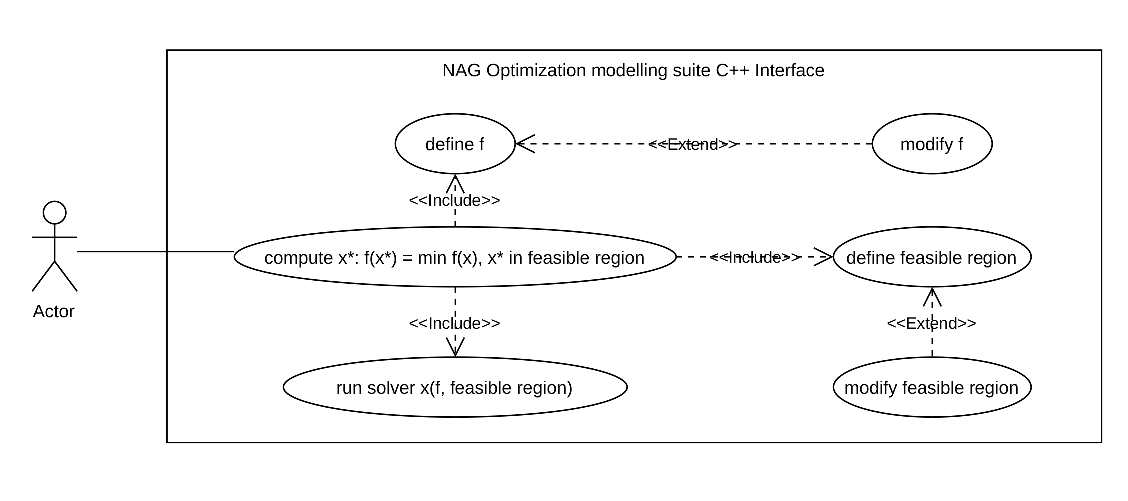
\includegraphics[width=\textwidth]{use case.pdf}
\caption{\small Use Case Diagram}
\end{figure}
\newline
The use case diagram shows how the interface processes this task of solving an optimization problem. To find an extreme of the function $f$, it defines the function and the feasible region, which could be modified later if needed, then chooses a certain solver to compute the extreme $x^{*}$. The user does not have to specify what type of problem it is (linear or non-linear), nor choose the right solver themself to solve it. 
\newpage

\section{Essential Technical Background}
Our C++ interface is based on the NAG Library, specifically the NAG optimization modelling suite, and an experimental C++ interface written by NAG, supplied as a series of header files and provides routines for solving mathematical optimization problems with various solvers.
\subsection{Concept of Optimization Problems}
An optimization problem\cite{nag} can be defined as:
$${\displaystyle {\begin{aligned}
&{\operatorname{minimize}} &&f(x)\\ &{\operatorname{subject\; to}}&& \mathit x \in \mathit{F}\end{aligned}}}$$ 
where x denotes the decision variables, f(x) the objective function and \textit{F} the feasibility set. We assume that $\mathit{F} \subset \mathbb{R}^n$. The goal here is to find the global minimum of a function in its given feasibility set. \\
\newline
Optimization problems can be classified into different categories based on various criteria:
\begin{enumerate}
\item Type of objective function: 

Recognizing the type of the objective function assists in deciding which solver should be used on the problem. In our case, we separate the objective functions into linear and noninear ones. \\
A \textbf{linear} objective function has the form $${\displaystyle f(x) = c^T x + c_0 , c  \in \mathbb{R}^n,}$$ which is linear in all variables. \\
A \textbf{nonlinear} objective function has no special structure, to which an example is the Rosenbrock function\footnote{\tt \url{https://www.sfu.ca/\~ssurjano/rosen.html}}: $${\displaystyle f(x)=(1-{x_1})^2+100 \cdot ({x_2}-{x_1}^2)^2.}$$ 
\item Type of constraints: 

Playing an important role in categorizing an optimization problem is its type of constraint, of which there are several. \\
For \textbf{unconstrained} problems, there are no restrictions on the choice of the variable ${\displaystyle x}$ as long as it belongs to its feasible region. \\
\textbf{Simple bounds} have a general form of  $${\displaystyle l_x \leq x \leq u_x,}$$ where ${\displaystyle l_x }$ and ${\displaystyle u_x}$ are n-dimensional vectors.\\
For \textbf{linear constraints}, the constraint function is linear in all variables and bounded. They are usually formed as:  $${\displaystyle l_B \leq B_x \leq u_B,}$$ where B is a general ${\displaystyle m_B}$ x n rectangular matrix and ${\displaystyle l_x }$ and ${\displaystyle u_x}$ are n-dimensional vectors.\\
\textbf{Nonlinear constraints} are defined as nonlinear functions and bounds, which have the form: $${\displaystyle  l_g \leq g(x) \leq u_g.}$$
\end{enumerate}
With the objective functions and constraints classified, they can be combined to define specific optimization problems, such as Linear- and Nonlinear- Programming, Quadratically Constrained Quadratic Programming, Least Squares, and etc. In this project, we focus on the following two typical classes: 
\begin{itemize}
\item A \textbf{Linear Programming (LP)} problem is made of linear objective function, linear constraints and simple bounds. It has a general form of: 
$${\displaystyle {\begin{aligned}
&{\underset{x\in \mathbb{R}^n}{\operatorname{minimize}} }&&c^Tx\\&{\operatorname{subject\; to}}&& l_B \leq Bx \leq u_B,\\&&&l_x \leq x \leq u_x.\end{aligned}}}$$ 
\item \textbf{Nonlinear Programming (NLP)} problems are more general with a nonlinear objective function and any of the nonlinear, quadratic, linear or bound constraints, which can be written as follows:
$${\displaystyle {\begin{aligned}
&{\underset{x\in \mathbb{R}^n}{\operatorname{minimize}} }&&f(x)\\ &{\operatorname{subject\; to}}&& l_g \leq g(x) \leq u_g,\\&&&l_B \leq Bx \leq u_B,\\&&&l_x \leq x \leq u_x.\end{aligned}}}$$ 
\end{itemize}

\subsection{NAG Library}
The NAG Library\footnote{\tt https://www.nag.com/content/nag-library} is a comprehensive collection of routines for the solution of numerical and statistical problems, comparable to FICO Xpress Optimization\footnote{\tt https://www.fico.com/en/products/fico-xpress-optimization} or Gurobi\footnote{\tt https://www.gurobi.com/}.\\
\newline
The NAG optimization modelling suite (NOMS)\footnote{\tt https://www.nag.com/numeric/nl/nagdoc\_latest/clhtml/e04/e04intro.html\#optsuite} is a part of the NAG Library, and is a suite of routines which allows the user to define and solve various optimization problems in a uniform manner, whose key features are that the definition of the optimization problem and the call to the solver are separated so that it is possible to set up a problem in the same way for different solvers and that the problem representation is built up from basic components (building blocks).\\
\newline
The NAG library (specifically the optimization modelling suite) is available in several languages, including Fortran, C, and an experimental C++ interface\footnote{\tt https://www.nag.com/content/nag-library-c-plusplus} that is hard to use. A C++ layer is to be built on top of the given C++ interface, offering the user easier access to the library by writing more simple code. This C++ interface also utillizes dco/c++ for additional functions not existing in the previous one.
\begin{figure}[h]
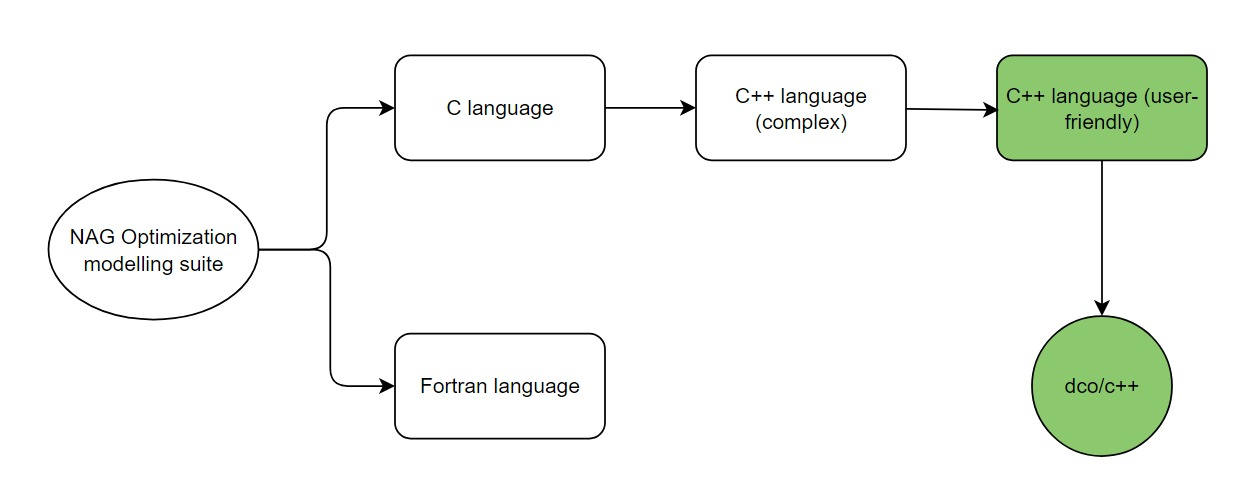
\includegraphics[width=\textwidth]{layering.jpeg}
\caption{\small C++ Interface layering}
\end{figure}

\subsection{dco/c++}
dco/c++\footnote{\tt https://www.nag.com/content/algorithmic-differentiation-software} is an operator-overloading Algorithmic Differentiation Tool, that can compute derivatives of an arbitrary order with machine precision. In this project, it is used to perform automatic differentiation to obtain the required derivative information, as well as determine the linearity of the problem constraints.

\section{System Requirements}
The following system requirements are introduced in two parts: functional and nonfunctional. 
\begin{itemize}
\item \textbf{Functional:}

The interface is to define optimization problems, including the ability to define and modify the objective and/or constraint functions. Moreover, it is to be able to compute derivatives automatically, recognize linear constraints and also modify the problem to reflect their linearity. To solve the optimization problem, the interface is to choose on its own, or, alternatively the user can manually select one from the three solvers: e04mt, e04kf, and e04st. 

\item \textbf{Nonfunctional:}

The interface should have the NOMS and the pre-existing C++ interface as its backend. The interface is to be implemented in C++ using object-oriented programming, tested with CTest and GoogleTest and documented with Doxygen. The automatic computation of derivatives and recognisation of linear contraints is to be done with dco/c++. 
\end{itemize}

\chapter{Design} \label{ch:design}
This chapter contains UML diagrams describing the interface and explains how it was designed.
\section{Class Model}
Depicted in the following pages are the class diagrams and an activity diagram of the interface. \\\\
Figures 2.1 to 2.4 shows how the interface is constructed. An explaination for how these design decisions were made is given in section 2.2. \\\\
Figure 2.5 visualizes the typical operation of the interface. A \texttt{Problem} is first defined and then given over to the \texttt{Solver}. The \texttt{Solver} as well as the \texttt{MonitorOption}'s parameters are tweaked (\textit{configure} in the diagram) according to the user's needs, then finally \texttt{Solver} solves and prints the solution to the optimization problem.
\begin{figure}[!hp]\centering
\makebox[\textwidth]{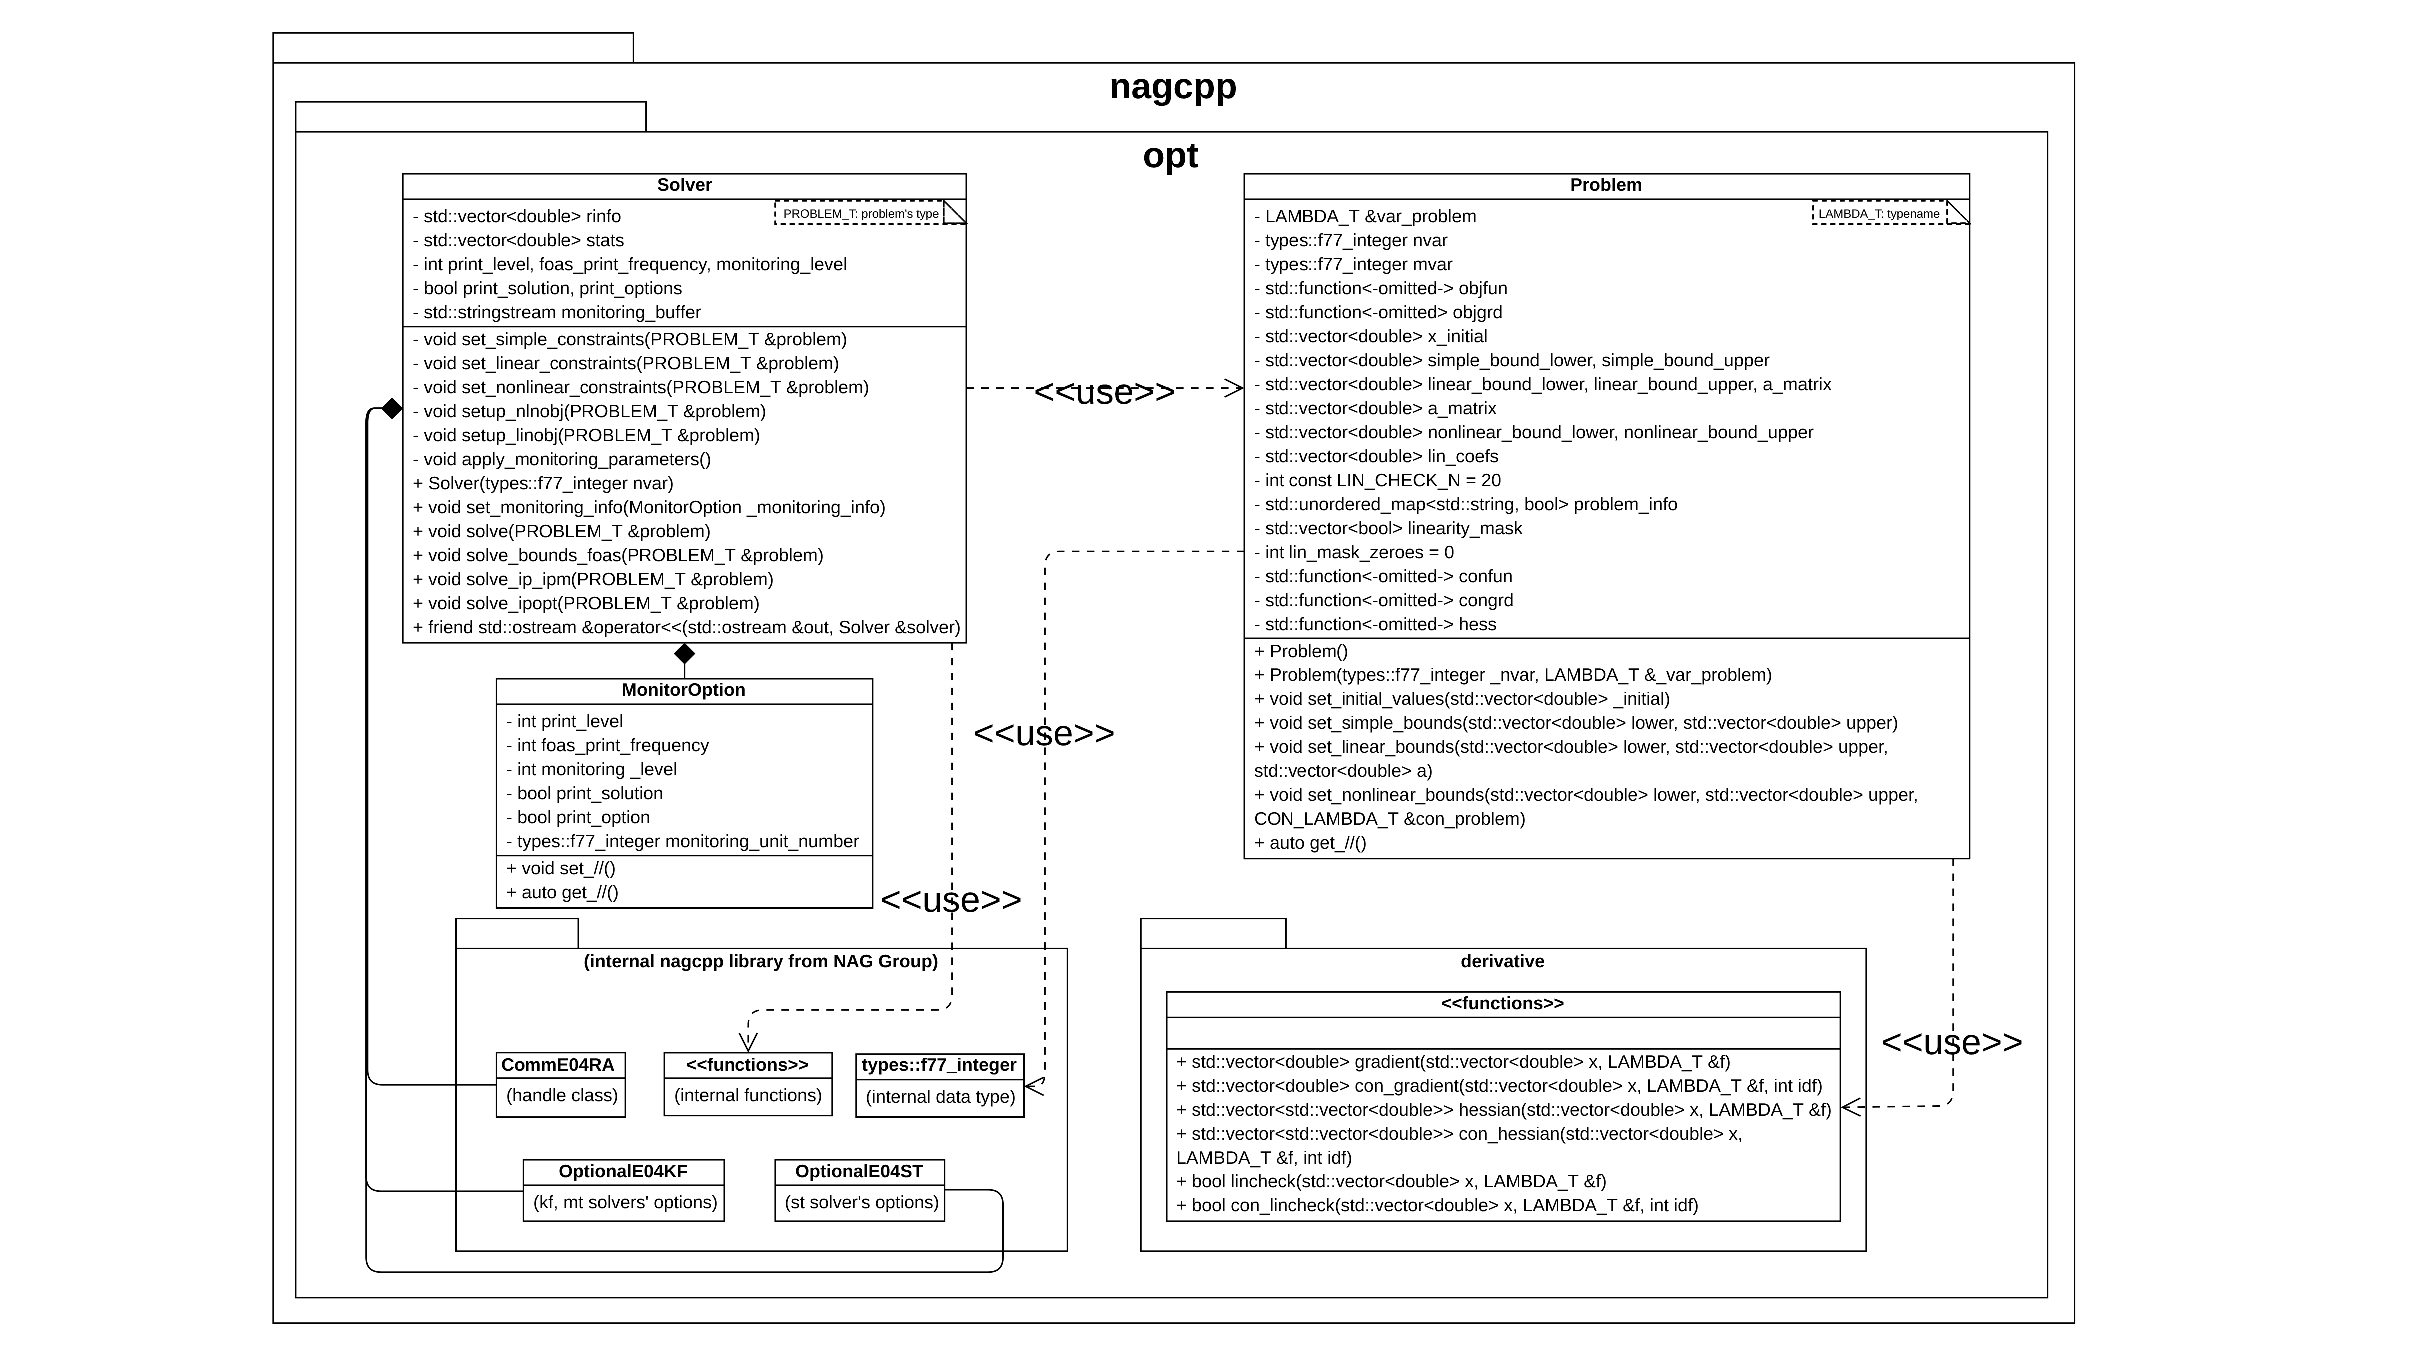
\includegraphics[width=\paperwidth]{class diagram.pdf}}
\caption{Class Diagram}
\end{figure}
\begin{figure}[!htbp]\centering
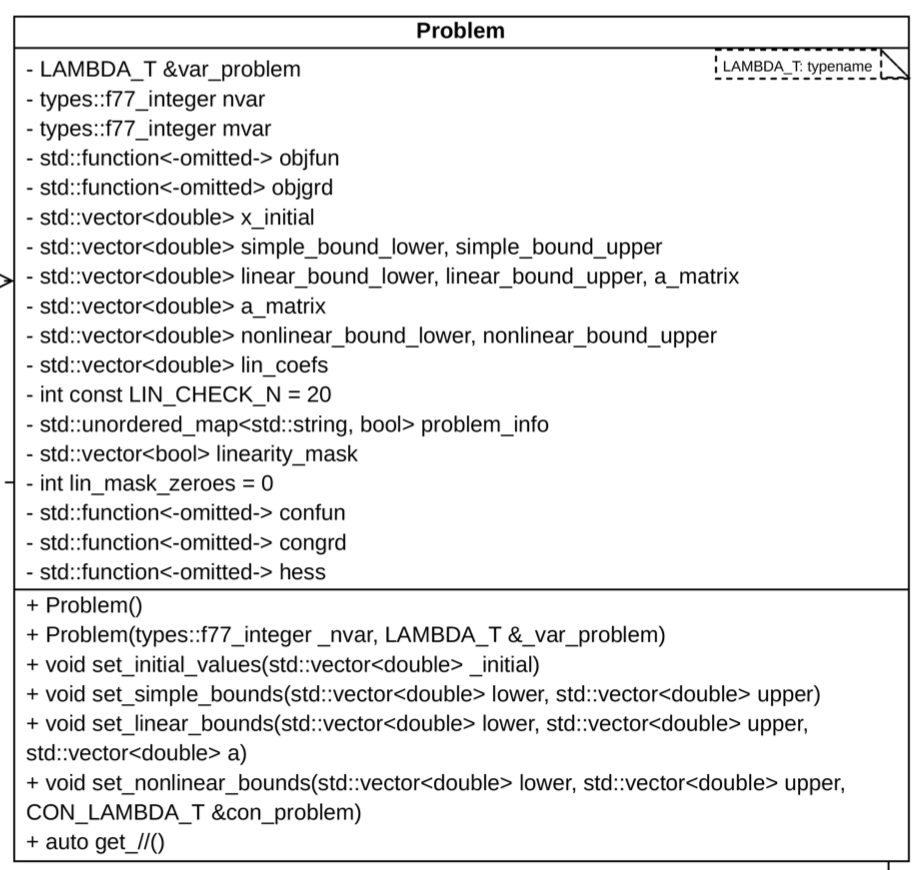
\includegraphics[width=\textwidth]{class problem.png}
\caption{Class Diagram - \tt Problem}%you could add longer caption here if you want, in case the addtional text messes up the layout
\end{figure}
\begin{figure}[!htbp]\centering
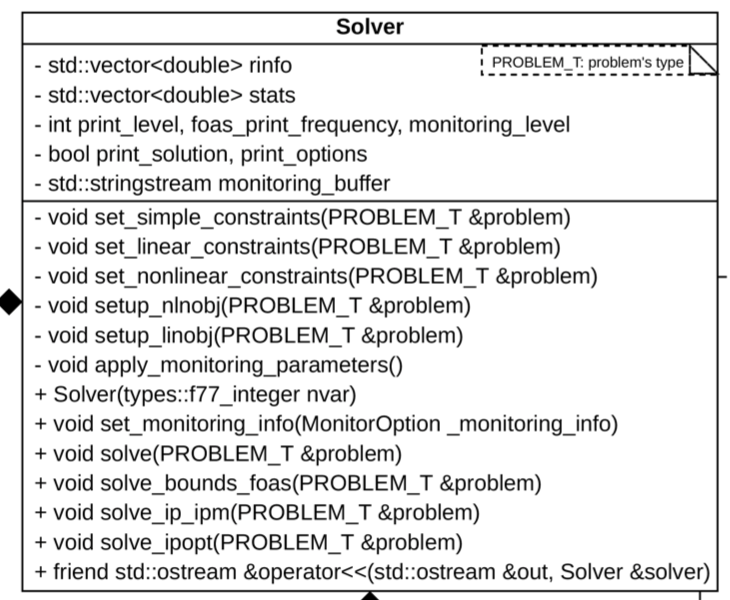
\includegraphics[width=\textwidth]{class solver.png}
\caption{Class Diagram - \tt Solver}
\end{figure}
\begin{figure}[!htbp]\centering
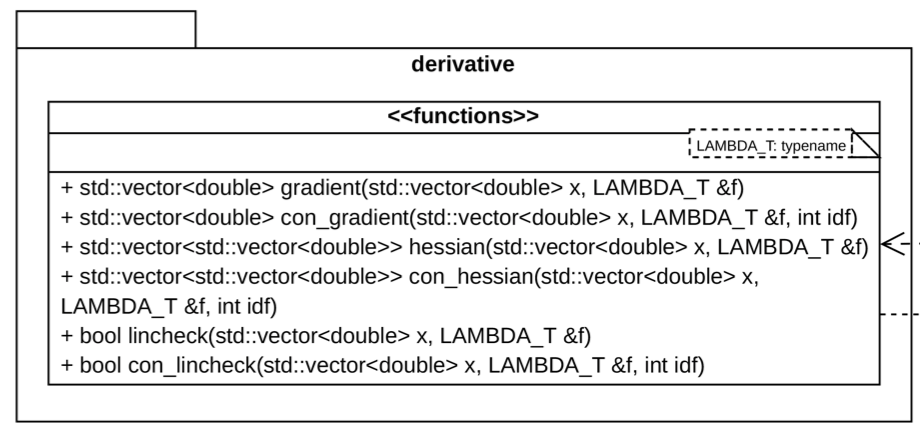
\includegraphics[width=\textwidth]{class derivative.png}
\caption{Class Diagram - \tt derivative}
\end{figure}
\begin{figure}[!htbp]\centering
\makebox[\textwidth]{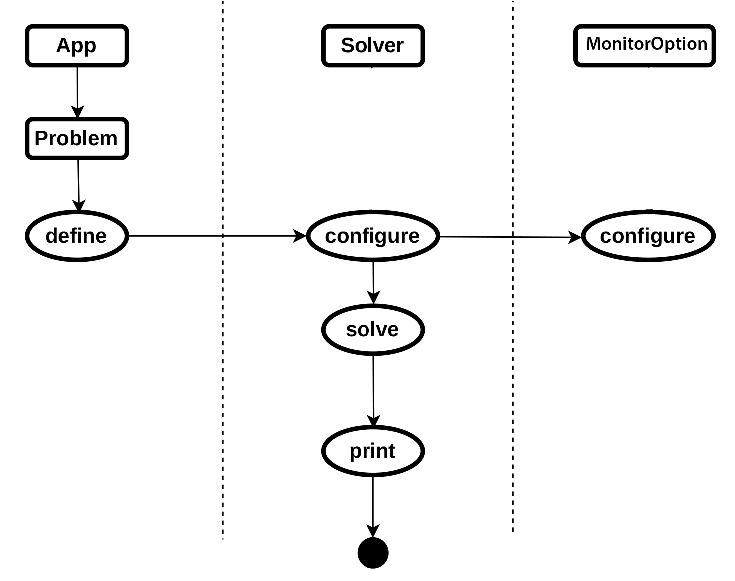
\includegraphics[width=0.8\paperwidth]{Class Model - Optimize function.pdf}}
\centering
\caption{Class Model - Optimize function}
\end{figure}
\newpage


\section{Class Design}
For our interface, we attempted to come up with a design that not only is as user-friendly as possible but also meshes well with the backend C++ interface for the NAG Library and specifically NOMS. To this goal, we have taken inspiration from softwares such as Gurobi and FICO Xpress Optimization, which are themselves commercially available optimization solvers.\\
\newline
The aforementioned backend interface uses a communicator class called \texttt{CommE04RA}, to which practically everything pertaining to the operation of the program must be assigned: all problem definitions such as the bounds of the feasible region and their linearity, to the various solver’s settings like desired accuracy and level of monitoring are contained within this monolith of a class. \\
\newline
Moreover, as perhaps a vestigial trait from its C background, the interface has no classes nor class methods. Everything the user could possibly do are done through functions, i.e. the \texttt{CommE04RA} class and a whole set of of auxiliary data must always be explicitly passed around into functions, resulting in some very awkward function calls such as\footnote{\tt The CommE04RA class is referred to here as handle}:
\begin{lstlisting}[basicstyle=\normalsize]
nagcpp::opt::handle_solve_bounds_foas(handle, 
					objfun, 
					objgrd, 
					nullptr, 
					x, 
					rinfo, 
					stats, 
					opt);
\end{lstlisting}
just for invoking one of the simplest solvers available in the old interface. For a first-time user, this can be very abstruse, as we have experienced firsthand ourselves in the undertaking of this project. Further contributing to the code bloat the user has to write is the fact that the manual computation and entry of the derivatives is required for selecting solvers, prone to calculational or typographical mistakes and potentially slowing down said solvers.\\
\newline
Our final design addresses all of these issues by first and most importantly splitting up the communicator class into two classes- \texttt{Solver} and \texttt{Problem}, each of which is populated with class methods, allowing for cleaner code writing. The supplementary data found in the example shown above such as \texttt{rinfo} and \texttt{stats} now also exist inherently within these classes as well. Beyond that, a \texttt{MonitorOption} class is written to hold some of the parameters determining what should be printed out when running the solvers. \\
\newline
This logical regrouping of the various elements offers the user a clearer overview when reading and writing programs with our new interface. We additionally employ the use of dco/c++ in the form of the package \texttt{derivative} to also determine the derivatives automatically, and now the user has but to define the objective and/or constraint functions. The previous verbose function call is reduced to be simply: 
\begin{lstlisting}[basicstyle=\normalsize]
solver.solve(problem);
\end{lstlisting}

\chapter{Implementation} \label{ch:implementation}
This chapters goes into details about how the interface was exactly implemented, how it was tested, as well as potential points for improvement.
\section{Development Infrastructure}
The set of infrastructure we utilized has been entirely and directly recommended to us by the project task description, as seen in the non-functional requirements in section 1.3. \\
\newline
Although our back-end, the NAG Library and its relatively hard-to-use C++ interface, is available for the two major operating systems Windows and Linux, we decided to target the later one, as this version brings with it many quality-of-life advantages over the Windows one. It also means that the work is contained in a singular consistent environment, namely the Virtual Machine provided by the SEP course. Correspondingly, we used the Linux version of dco/c++ for the automatic computation of derivatives. The exact model numbers are \textit{nll6i285bl} for the NAG Library, \textit{28.5.0.0} for the pre-existing C++ interface, and \textit{dcl6i37ngl\_v370} for dco/c++. Some of the standard C++ libraries are additionally present in the projects, most important of which is \texttt{functional}, which facilitates the functional programming style found in our implementation.\\
\newline
We selected C++ 20, the latest stable version, as our programming language for the project, whose numerous modern features assisted in simplifying the interface for end-users. We used gcc accordingly as our compiler of choice thanks to its support for selected version C++. CMake then comes into play for the build system, as its support of scripting heavily eases up the otherwise overly complicated build commands to be run, as well as allows the user to easily add new custom programs at a whim. To help the user write such programs, documentation was automatically generated with the help of Doxygen.\\
\newline
Of great assistance to us in writing and debugging the code was the GNU Debugger and Valgrind, keeping the program free of any memory leak and invalid memory access. The powerful combination detected several subtle errors in the coding process, which resulted from unforeseeable side-interactions between the many functions present in the interface. CTest was additionally used in tandem with GoogleTest to verify that all behaviors were intended, upon which will be expanded in section 3.3. Finally, Git is used for version control.


\section{Source Code}
The source code is hosted on a Git repository\footnote{\tt https://git.rwth-aachen.de/tranmankhang1705/nag-optimization-modelling-suite-ui}. We have decided to not explicitly put the source code in this report. For access to the Git repository please contact us and make a request- we will try to reply as soon as possible. Our contact informations are found in \texttt{README.md}.
\subsection{File Structure Overview}
We divided the project file into several subdirectories. Most importantly, the interface library is contained within \texttt{/include}, meanwhile the pre-existing NAG Library C++ interface and its license keys are found within \texttt{/thirdParty/nag.cpp} and \texttt{/license} respectively. \texttt{/examples}, \texttt{/caseStudies}, and \texttt{/tests} contain what their names would suggest. \\
\newline
The following shows the file structure in the form of a hierarchy tree:
\begin{lstlisting}[numbers=none]
include (C++ header files)
  |-- derivative.hpp
  |-- nag_cpp.hpp
  |-- problem.hpp
  |-- solver.hpp
caseStudies (directories containing various problem cases)
cmake (auxiliary files required for building and testing with CMake)
  |-- FindNAG_dco_cpp.cmake
  |-- FindNAG_Library.cmake
CMakeLists.txt (used for building and testing)
examples (directories containing various example programs)
tests (with googletest and ctest)
  |-- CMakeLists.txt
  |-- test_dco
  |-- test_linearity
  |-- test_set_get
thirdParty/nag_cpp (NAG C++ interface from NAG group)
doc
  |-- talk (slides)
  |-- report (this report)
  |-- caseStudiesVisualisation
  |-- briefing.pdf (assignment)
  |-- userGuide.pdf
license
  |-- nag.key
README.md
\end{lstlisting}

\subsection{Source Code Structure Overview}
The first major class is \texttt{Problem}. Its members consist of every parameter of the optimization problem to be solved, from the objective functions and the various derivatives, to the bounds of the feasible region as well as the constraint functions and their linearity. The objective function and constraint function are type-templated, enabling the usage of data types beside the standard ones. dco/c++ is employed as the \texttt{derivative} package here by \texttt{Problem} to perform automatic derivativation on these functions. The class allows the user to interact with these parameters through a series of set and get functions.\\
\newline
\texttt{Problem} is passed into the second major class named \texttt{Solver}. It holds the communicator class \texttt{CommE04RA} used in the back-end NAG Library interface, which will thus be referred to as \texttt{handle}. All of \texttt{Problem}’s parameters are given over to \texttt{handle} using private wrapper functions held by \texttt{Solver}. \texttt{Solver} additionally contains settings specifying the error tolerance of the numerical result as well as printing options with the assistance of the helper class \texttt{MonitorOption}, all of which are also passed into \texttt{handle}. Last and certainly not least, \texttt{Solver} houses the eponymous \texttt{solve(...)} function, which automatically analyzes the problem’s parameters so as to choose most optimal solvers from the three present in the interface.

\subsection{dco/c++}
Automatic derivation is performed by dco/c++ for the purpose of calculating the gradient, the Hessian matrix and the linearity of any given function. An example of how the gradient is determined is shown below:
\begin{lstlisting}[basicstyle=\normalsize]
template <typename LAMBDA_T>
std::vector<double> gradient(std::vector<double> x, LAMBDA_T &f)
{
	std::vector<double> grad(x.size());
	using type = dco::gt1s<double>::type;
	std::vector<type> ax(x.begin(), x.end());
	for (std::size_t i = 0; i < x.size(); ++i)
	{
		dco::derivative(ax[i]) = 1.0;
		type ay = f(ax);
		grad[i] = dco::derivative(ay);
		dco::derivative(ax[i]) = 0.0;
	}
	return grad;
}
\end{lstlisting}
For each of these functions there are 2 versions, one for the objective function (${\displaystyle \mathbb{R}^n \rightarrow \mathbb{R}}$) and one for the given constraints (${\displaystyle \mathbb{R}^n \rightarrow \mathbb{R}^m}$), as the codomain of the constraints can be multidimensional. The gradient is computed with the first tangent method. The Hessian matrix, on the other hand, requires derivatives of the second order, so both the first tangent and second adjoint methods are used to acquire it. As for examining the linearity, only entries on the diagonal of the Hessian matrix are looked at. Because the diagonal elements of the Hessian matrix are second order derivatives of the functions, we check if those are equal to zero and then deduce if the function is linear or not.

\subsection{Code Documentation}
All codes are properly documented with Doxygen for the purpose of guiding the user, including comments for each parameter in every function. The same set of comments are found within the individual code files themselves, helping future developers further expand the interface. \\
\newline
An example: 
\begin{lstlisting}[basicstyle=\normalsize]
//! Objective function.
/*!
\param x vector of variable x.
\param y the value of objective function in x.
\param inform additional information.
*/
auto _objfun = [&_var_problem](auto const &x, auto &y, auto &inform)
{
	_var_problem(x, y);
};
this->objfun = _objfun;
\end{lstlisting}

\subsection{Points of Interest}
While the user is to define their objective functions and constraint functions as type-generic lambdas, they are internally stored within the \texttt{Problem} class as \texttt{std::functions}\footnote{\tt https://en.cppreference.com/w/cpp/utility/functional/function}. This is because even though two lambdas may take and return the same data type, the lambdas themselves could be of different types\footnote{\tt For further reference see: https://lesleylai.info/en/std-function/}, which creates potential conflicts in the back-end NAG C++ interface. \texttt{std::function} is therefore used to store them, as it is a type erasure object and provides a singular uniform runtime interface to the lambdas for the mentioned library. \\
\newline
We went into this with the mindset to simplify the interface as much as possible for the user. Thus, extra care was taken in writing the function\\ \texttt{Problem.set\_nonlinear\_bounds()}. An edge case can happen where the user incorrectly registers a set of constraint functions which are actually linear instead of non-linear, resulting in inefficient handling of the terms and consequently a less than optimal solving of the problem. Therefore, the function uses dco/c++ to check for the linearity of every given constraint function and sort them accordingly.\\
\newline
As alluded to above, modern C++ features were taken advantage of, one of them being the automatic class template type deduction. For a given objective function: 
\begin{lstlisting}[basicstyle=\normalsize]
auto test_problem = [](auto const &x, auto &y)
{
    y = pow(x[0], 2) + pow(x[1], 2);
};
\end{lstlisting}

The construction of the \texttt{Problem} class can written like so: 
\begin{lstlisting}[basicstyle=\normalsize]
nagcpp::opt::Problem problem(nvar, test_problem);
\end{lstlisting}

Even though \texttt{Problem} is a type-templated class, the user is spared from having to do any manual type declaration.

\subsection{Potential Improvements}
Although we have fulfilled all of the requirements stated by the project assignment, it is easy to imagine where the interface could still be expanded upon. The following points are outside of the scope of the project, but are still listed for potential future development. 
\begin{itemize}
\item We currently base our interface off of the experimental C++ interface already written by the NAG Group, which in itself calls on the C interface of the library. It is possible to base the interface directly off of the C interface. Conceptually this would remove the middleman so to speak, but requires a massive overhaul of our program.
\item Our interface allows for easy addition of new solvers, if they are available in the back-end library. We have currently implemented three solvers in the current project, but five solvers in total are present in the C++ interface we built on and additional seven solvers can be found in the original C one. These could and should be added to our work for the sake of completeness.
\item The linearity of the constraint functions could yet still be better leveraged. As it stands right now, even if a constraint function has but one nonlinear term, the entire function is treated as such, slowing down the solver:
\begin{lstlisting}[basicstyle=\normalsize]
auto constraint_problem = [](auto const &x, auto &y)
{
	y.resize(1);
	y[0] = 1 * x[0] + 2 * x[1] + 3 * x[2] + 4 * x[3] - 5 * pow(x[0], 2);
};
\end{lstlisting}
In this example, although only the last term is nonlinear, this causes the function to be classified as nonlinear. A better approach would be to separate the individual terms into whether they are linear or nonlinear and readjust the optimization problem’s definition accordingly, but this is yet to be achieved.
\end{itemize}


\section{Software Tests}
For the testing of our software, we used Valgrind\footnote{\tt https://valgrind.org} to make sure the program is free of memory leaks and invalid memory accesses and GoogleTest\footnote{\tt https://github.com/google/googletest} / CTest for unit tests. \\
We made use of the two assertions provided by GoogleTest\cite{googletest}: ASSERT and EXPECT, the former one generates fatal failure when the test fails which means the current function will then be aborted, while the latter one won't stop the process. When the test fails, GoogleTest prints out the assertion's source file and line number, along with a failure message which was customized in our cases. We designed our unit tests based on various granularities, each with at least three test functions together with a test fixture class to use the same data for independent unit tests, which are introduced as follows: 
\begin{itemize}
\item \textbf{Basic set/get routines} (\texttt{test\_set\_get.cpp}):\\
The basic set/get routines are tested for the following objects: simple bounds, number of variables and objective function. The test objects will be checked whether their values given by the get() function are the same as they are given by the users. For example: 
\begin{lstlisting}[basicstyle=\normalsize]
TEST_F(ProblemTest, NVarEQ)
{
	auto problem = make_problem(test_problem);
	ASSERT_EQ(nvar, problem.get_nvar()) << "nvar and problex.get_nvar are unequal";
}
\end{lstlisting}
\item \textbf{Derivatives computation} (\texttt{test\_dco.cpp}):\\
Objective and constraint gradients and the Hessian matrix computed by dco/c++ are tested respectively whether they are correct or not compared to the right values given manually. The following example tests the computation of the Hessian matrix: 
\begin{lstlisting}[basicstyle=\normalsize]
TEST_F(ProblemTest, HessianEQ)
{
	std::vector<std::vector<double>> y1 = {{-30, -24}, {-24, -42}};
	auto y2 = nagcpp::opt::derivative::hessian(x, test_problem_2);
	ASSERT_EQ(y1.size(), y2.size()) << "Vector y1 and vector y2 are of unequal length";
	for (int i = 0; i < nvar; ++i)
	{
		EXPECT_EQ(y1[i], y2[i]) << "Vector y1 and vector y2 differ at index " << i;
	}
}
\end{lstlisting}
\item \textbf{More complex linearity detection logic} (\texttt{test\_linearity.cpp}):\\
To test the linearity detection logic in the program, we have two test problems and two constraints as examples, one being linear and the other nonlinear. By checking the variable \texttt{getProbInfo}, we could test the problem's linearity detection and whether the corresponding boundary parameters to a test problem have been declared and correctly classified. For instance: 
\begin{lstlisting}[basicstyle=\normalsize]
TEST_F(ProblemTest, NonLinearProblemCheck)
{
	auto problem = make_problem(test_problem_1);
	auto getProbInfo = problem.get_problem_info();
	EXPECT_FALSE(getProbInfo["is_linear"]) << "Problem is linear";
}
\end{lstlisting}
This test above checks the linearity detection for nonlinear problems.
\end{itemize}

\chapter{Project Management} \label{ch:projectmanagement}
This chapter is about how we distributed the work among ourselves. \\\\
Our project workflow is divided into five phases in a time span of 6 months: analysis, design and implementation, testing, documentation and final report writing. \\
\begin{figure}[h!]
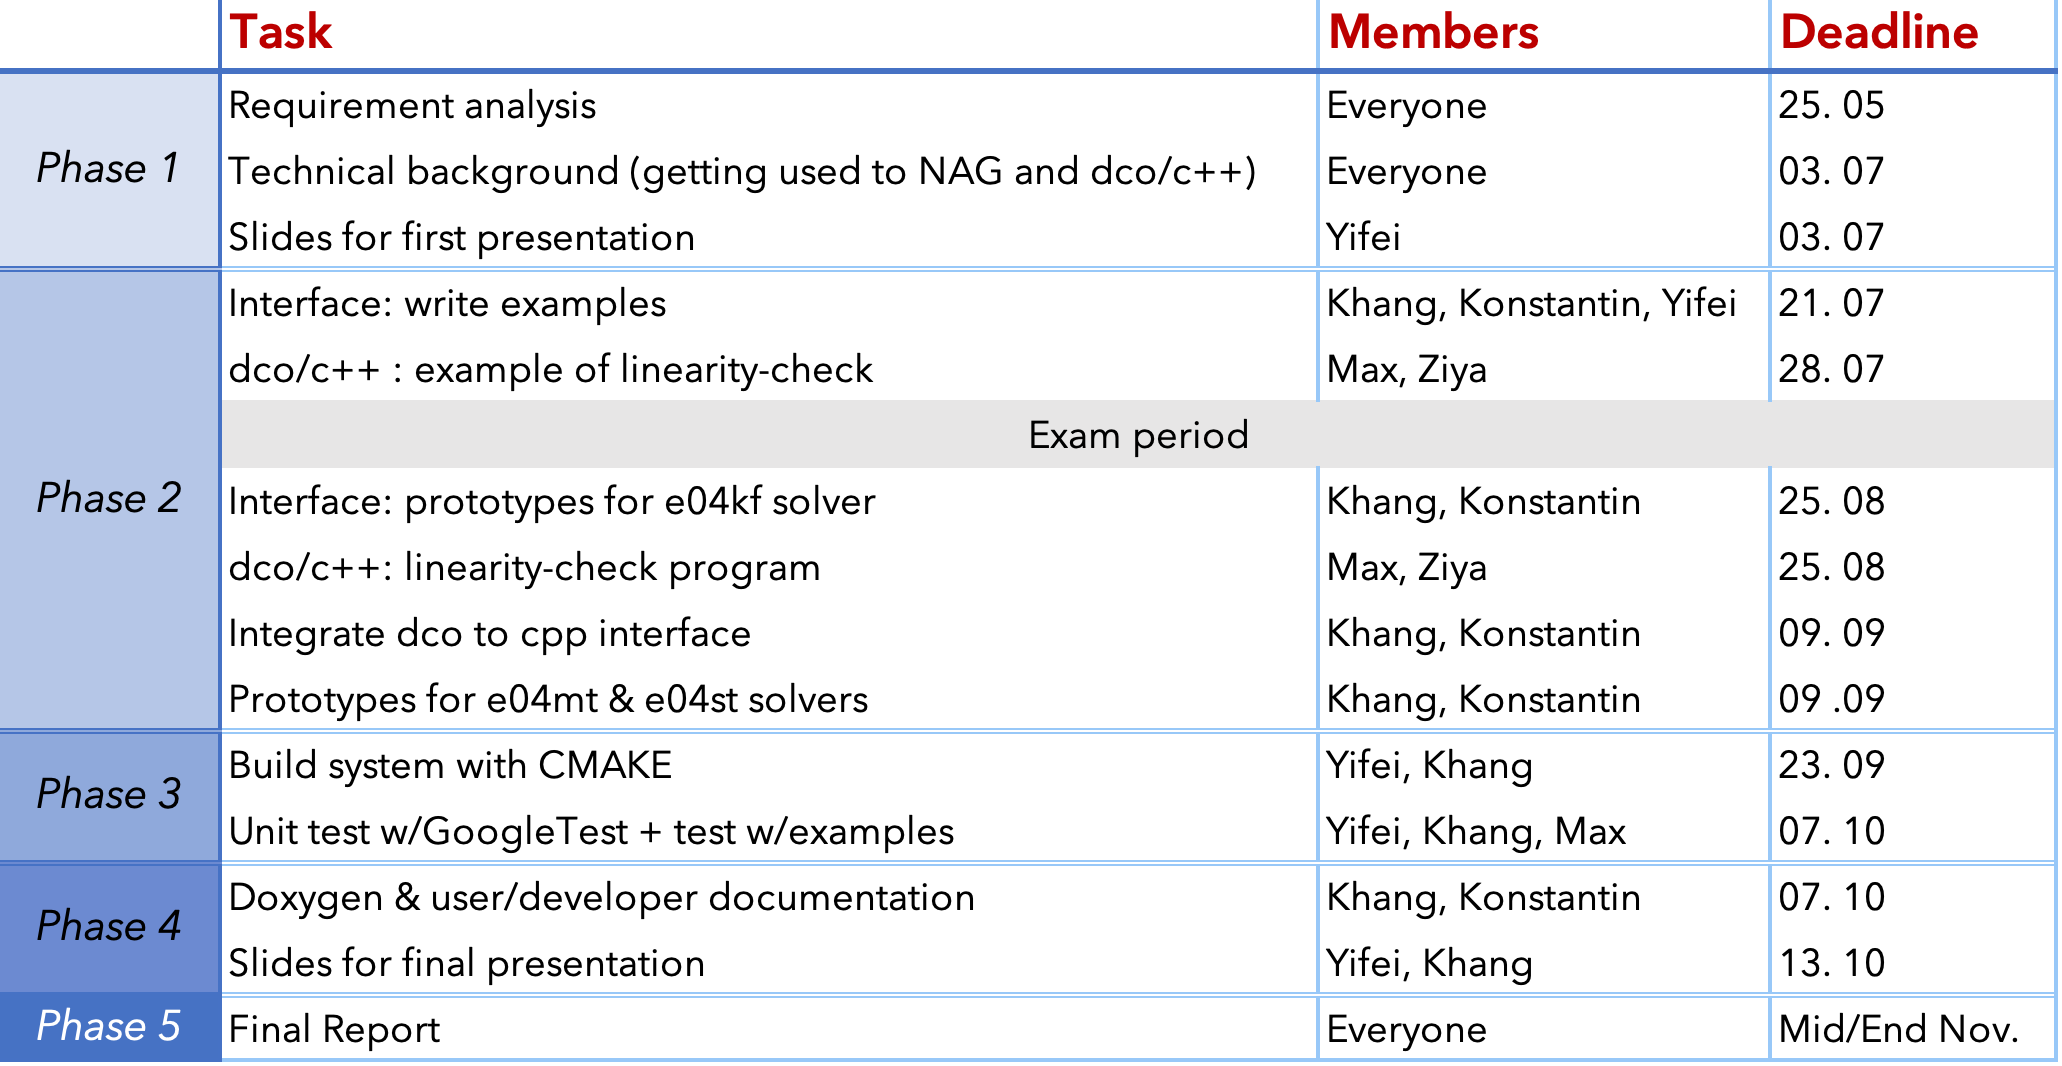
\includegraphics[width=\textwidth]{proj_management.png}
\caption{\small Project Management table}
\end{figure}
\newline
At the start of this project, we discussed and worked together on the requirement analysis and technical background so that everyone could have the basic understanding of the project assignment and also get to know the NAG library for later development. At the beginning of July, we then presented the requirement analysis of our project and came up with preliminary division of work for the rest of the phases. \\
\newline
In the design and implementation phase, Khang and Konstantin took charge of the main C++ interface (prototypes for the three solvers, etc.) and implemented the code in C++20 whilst Ziya was responsible for applying dco/c++ for automatic differentiation and linearity check. Despite the one-month-long exam period for all members, we still managed to stick to our time plan. \\
\newline
After the source code was implemented and ran successfully with all expected features, Yifei constructed a build system based with CMake which Khang then restructured. Meanwhile, Yifei and Khang looked into GoogleTest and CTest to create unit tests for the interface together with Valgrind to ensure it was free of memory leaks and invalid memory accesses. Max implemented three examples for each solver to ensure us the functionality of the interface. \\
\newline
Before the final presentation of the project, Khang and Konstantin worked on user and developer documentation with doxygen as they were the most familiar with the source code. With Khang summarizing and arranging the content of the presentation and report, Yifei made the slides in \LaTeX\ for both presentation and also the report of the project. \\
\newline
As a group, we kept our communication both internal and with our supervisor Johannes, managed the time and overcame exceptional situations such as sickness, which was precious experience in software development for all of us.\\
We sticked to our roles as originally planned and made sure to have both online group meetings every week to discuss and online meetings with our supervisor every two week to have them check on our progress so that everything was kept on track very well. To keep everything up-to-date on everyone's end, we made use of Git for software version control. As a prevention of unexpected circumstances, tasks were always assigned to a pair of our group members. If one person is unavailable, there is still another to continue the work, which turned out to be of much use.


\bibliographystyle{plain}
\bibliography{literature}

\appendix

\chapter{User Documentation} \label{ch:userdoc}
A stand-alone and more in-depth user documentation can be found under \\ \texttt{/doc/userGuide.pdf}. We include an abbreviated version of said documentation here.
\section{Building}
The location in which the interface directory is placed is referred to as \texttt{\$\{REPO\_DIR\}}. In an arbitrary directory, create a new directory ’build’ and move there:\\
\texttt{\# mkdir build \&\& cd build}\\
\newline
Run CMake to create the necessary make files, changing \texttt{\$\{HOME\}}, if an alternative installation directory for the NAG Library and dco/c++ was chosen beforehand:\\
\texttt{\# cmake \$\{REPO\_DIR\} -DNAG\_dco\_cpp\_DIR=\$\{HOME\}/NAG/dcl6i37ngl\_v370/ \\-DNAG\_Library\_DIR=\$\{HOME\}/NAG/nll6i285bl/}\\
\newline
To build, run:\\
\texttt{\# make} \\
\newline
It is possible to build individual examples, case studies and code tests by setting a target:\\
\texttt{\# make examples.xxx\\
\# make tests.xxx\\
\# make caseStudies.xxx}\\
to compile an arbitrary program from the \texttt{/examples}, \texttt{/tests}, or \texttt{/caseStudies} folder respectively.\\
\newline
To build and execute an example (in this case, e04kf), run the following:\\
\texttt{\# make examples.e04kf}\\
\newline
To build and execute your own programs, create a sub directory with an arbitrary \texttt{\$\{SUB\_DIR\_NAME\}} within \texttt{/examples} and place your programs there. Thus, run:\\
\texttt{\# make examples.\$\{SUB\_DIR\_NAME\}}\\
\newline
Note: A new sub directory is to be created for every program, as they can only contain one program each.

\section{Testing}
To run the code tests, run:\\
\texttt{\# ctest}

\section{Running}
To execute an example (here: e04kf), run the following:\\
\texttt{\# ./examples/examples.e04kf}\\
\newline
To execute your own programs, run:\\
\texttt{\# ./examples/examples.\$\{SUB\_DIR\_NAME\}}\\
\newline
Note: While using non-linear constraint function, make sure to resize the y-variable of the constraint function by its output dimension, e.g. for ${\displaystyle g: \mathbb{R}^n \rightarrow \mathbb{R}^m}$ type \texttt{y.resize(m)}. Consult section 5 of the documentation found under \\ \texttt{/doc/userGuide.pdf} for further information.


\end{document}

